\documentclass[8pt,titlepage]{article}

\usepackage[T1]{fontenc}
\usepackage[polish]{babel}
\usepackage[utf8]{inputenc}
\usepackage{lmodern}
\usepackage{enumerate}
\usepackage{color}
\usepackage{graphics}
\setlength{\parindent}{0pt}
\selectlanguage{polish}
\title{\textcolor{red}{Ordo Missae}}
\author{Stałe części Mszy Świętej\\według nadzwyczajnej formy rytu rzymskiego }
\date{}
\makeatletter
\def\@makechapterhead#1{%
	\vspace*{50\p@}%
	{\parindent \z@ \raggedright \normalfont
		\interlinepenalty\@M
		\Huge\bfseries  \thechapter.\quad #1\par\nobreak
		\vskip 40\p@
}}
\makeatother

\usepackage{enumitem}
\newlist{myDescr}{itemize}{1}
\setlist[myDescr,1]{%
	label={},
	noitemsep,
	leftmargin=10pt,
}
\setlist[myDescr]{%
	label={},
	noitemsep,
}

\usepackage{parcolumns}
\newcommand{\latinS}[1]{\colchunk{\begin{myDescr}\item[\textbf{S.}]{#1}\end{myDescr}}}
\newcommand{\latinM}[1]{\colchunk{\begin{myDescr}\item[\textbf{M.}]{#1}\end{myDescr}}}
\newcommand{\latinV}[1]{\colchunk{\begin{myDescr}\item[\textbf{V.}]{#1}\end{myDescr}}}
\newcommand{\latinR}[1]{\colchunk{\begin{myDescr}\item[\textbf{R.}]{#1}\end{myDescr}}}
\newcommand{\latin}[1]{\colchunk{\begin{myDescr}\item{#1}\end{myDescr}}}
\newcommand{\pol}[1]{\colchunk{\begin{myDescr}\item{#1}\end{myDescr}}\colplacechunks}
\newcommand{\polV}[1]{\colchunk{\begin{myDescr}\item[\textbf{V.}]{#1}\end{myDescr}}\colplacechunks}
\newcommand{\polR}[1]{\colchunk{\begin{myDescr}\item[\textbf{R.}]{#1}\end{myDescr}}\colplacechunks}
\newcommand{\polK}[1]{\colchunk{\begin{myDescr}\item[\textbf{K.}]{#1}\end{myDescr}}\colplacechunks}
\newcommand{\polW}[1]{\colchunk{\begin{myDescr}\item[\textbf{W.}]{#1}\end{myDescr}}\colplacechunks}

\newcommand{\rub}[1]{\textcolor{red}{#1}}
\newcommand{\negr}[1]{\textbf{#1}}

\usepackage[raggedright]{titlesec}

\usepackage{titlesec}
\titleformat{\section}
{\Large\bfseries} % format
{}                % label
{0pt}             % sep
{\Huge\centering}           % before-code
\titleformat{\subsection}
{\Large\bfseries} % format
{}                % label
{0pt}             % sep
{\LARGE\centering}           % before-code
\titleformat{\subsubsection}
{\Large\bfseries} % format
{}                % label
{0pt}             % sep
{\Large}           % before-code

\usepackage{geometry}
\newgeometry{tmargin=3cm, bmargin=3cm, lmargin=3cm, rmargin=3cm}

\begin{document}
	\maketitle
	\clearpage
	\tableofcontents
	\clearpage
	
	\section{MSZA KATECHUMENÓW}
	
	\subsection{CZĘŚĆ PIERWSZA}
	
	\subsubsection{Asperges --- Aspersja}
	\negr{(tylko w mszach uroczystych)}
	
	\subsubsection{Psalm wstępny}
	\begin{parcolumns}[colwidths={2=3 in},nofirstindent]{2}
		\rub{Kapłan stanąwszy u stopni ołtarza, żegna się znakiem krzyża i odmawia antyfonę:}
		
		\latinS{In nomine Patris, (+) et Filii, et Spiritus Sancti. Amen.\\Introibo ad altare Dei.}
		\polK{W imię Ojca + i Syna i Ducha Świętego. Amen.\\Przystąpię do ołtarza Bożego.}
		\latinM{Ad deum qui laetificat iuventutem meam.}
		\polW{Do Boga, który jest weselem moim od młodości.}

		\negr{Psalm 42}

		\latinS{Iudica me Deus, et discerne causam meam de gente non sancta: ab homine iniquo et doloso erue me.}
		\polK{Bądź mi sędzia, o Boże i rozsądź sprawę moją z narodem bezbożnym; wybaw mnie od człowieka niedobrego i fałszywego.}
		\latinM{Quia tu es Deus fortitudo mea: quare me repulisti, et quare tristis incedo, dum affligit me inimicus?}
		\polW{Wszak Ty jesteś, o Boże mocą moją; czemu mnie odrzucasz i czemu smutny chodzę, gdy nieprzyjaciel mnie nęka?}
		
		\latinS{Emitte lucem tuam, et veritatem tuam: ipsa me deduxerunt, et adduxerunt in montem sanctum tuum, et in tabernacula tua.}
		\polK{Ześlij światłość Swoją i prawdę Swoją; one mnie poprowadzą i przywiodą na góre święta Twoją, aż do przybytków Twoich.}
		\latinM{Et introibo ad altare Dei: ad Deum qui laetificat iuventutem meam.}
		\polW{I przystąpię do ołtarza Bożego, do Boga, który jest weselem moim od młodości}
		
		\latinS{Confitebor tibi in cithara Deus, Deus meus: quare tristis es anima mea, et quare conturbas me?}
		\polK{Chwalić Cię będę przy dźwiękach cytry, Boże, Boże mój; czemuś smutna, duszo moja, i czemu mnie trwożysz?}
		\latinM{Spera in Deo, quoniam adhuc confitebor illi: salutare vultus mei, et Deus meus.}
		\polW{Ufaj Bogu, albowiem jeszcze uwielbiać Go będę, jako Zbawcę i Boga mego.}
		
		\latinS{Gloria Patri, et Filio, et Spiritu Sancto.}
		\polK{Chwała Ojcu i Synowi, i Duchowi Świętemu}
		\latinM{Sicut erat in principio, et nunc, et semper, et in saecula saeculorum. Amen.}
		\polW{Jak było na początku, teraz i zawsze i na wieki wieków. Amen.}
		
		\latinS{Introibo ad altare Dei}
		\polK{Przystąpię do ołtarza Bożego}
		\latinM{Ad Deum qui laetificat iuventutem meam.}
		\polW{Do Boga, który jest weselem moim od młodości}
	\end{parcolumns}	
	
	\subsubsection{Confiteor --- Spowiedź powszechna}
	\begin{parcolumns}[colwidths={2=3 in},nofirstindent]{2}
		\rub{Wobec Boga i Kościoła powszechnego oskarżamy się publicznie o winy nasze, abyśmy tym głębszą w sobie obudzili skruchę}
		
		\latinS{Adiutorium nostrum (+) in nomine Domini.}
		\polK{Wspomożenie nasze (+) w Imieniu Pana.}
		\latinM{Qui fecit caelum et terram.}
		\polW{Który stworzył niebo i ziemię.}
	
		\rub{Kapłan głęboko pochylony odmawia spowiedź ogólną}
	
		\latinS{Confiteor Deo omnipotenti, beatae Mariae semper Virgini, beato Michaeli Archangelo, beato Ioanni Baptistae, sanctis Apostolis Petro et Paulo, omnibus Sanctis et vobis fratres, quia peccavi nimis cogitatione, verbo, et opere: mea culpa, mea culpa, mea maxima culpa. Ideo precor beatam Mariam semper Virginem, beatum Michaelem Archangelum, beatum Ioannem Baptistam, sanctos Apostolos Petrum et Paulum, omnes Sanctos, et vos fratres, orare pro me ad Dominum Deum nostrum.}
		\polK{Spowiadam się Bogu wszechmogącemu, Najświętszej Maryi zawsze Dziewicy, świętemu Michałowi Archaniołowi, świętemu Janowi Chrzcicielowi, świętym Apostołom Piotrowi i Pawłowi, wszystkim Świętym i wam, bracia, że bardzo zgrzeszyłem, myślą, mową i uczynkiem: Ksiądz uderza się trzykroć w piersi moja wina, moja wina, moja bardzo wielka wina. Przeto błagam Najświętszą Maryję zawsze Dziewicę, świętego Michała Archanioła, świętego Jana Chrzciciela, świętych Apostołów Piotra i Pawła, wszystkich świętych, i was, bracia, abyście się za mnie modlili do Pana Boga naszego.}
	
		\rub{Ministrant i wierni proszą za kapłanem}
	
		\latinM{Misereatur tui omnipotens Deus, et dimissis peccatis tuis, perducat te ad vitam aeternam.}
		\polW{Niech się zmiłuje nad tobą Bóg wszechmogący, a odpuściwszy ci grzechy twoje, niech cię doprowadzi do żywota wiecznego.}
		\latinS{Amen}
		\polK{Amen}
	
		\rub{Ministrant i wierni mówią pochyleni}
	
		\latinM{Confiteor Deo omnipotenti, beatae Mariae semper Virgini, beato Michaeli Archangelo, beato Ioanni Baptistae, sanctis Apostolis Petro et Paulo, omnibus Sanctis et tibi, Pater, quia peccavi nimis cogitatione, verbo, et opere:}
		\polW{Spowiadam się Bogu wszechmogącemu, Najświętszej Maryi zawsze Dziewicy, świętemu Michałowi Archaniołowi, świętemu Janowi Chrzcicielowi, świętym Apostołom Piotrowi i Pawłowi, wszystkim Świętym i tobie, Ojcze, żem zgrzeszył bardzo myślą, mową i uczynkiem:}
	
		\rub{Uderzyć się trzykroć w piersi mówiąc:}
	
		\latin{mea culpa, mea culpa, mea maxima culpa. Ideo precor beatam Mariam semper virginem, beatum Michaelem archangelum, beatum Ioannem Baptistam, sanctos Apostolos Petrum et Paulum, omnes Sanctos, et te, Pater, orare pro me ad Dominum Deum nostrum.}
		\pol{moja wina, moja wina, moja bardzo wielka wina. Przeto błagam Najświętszą Maryję zawsze Dziewicę, świętego Michała Archanioła, świętego Jana Chrzciciela, świętych Apostołów Piotra i Pawła, wszystkich świętych, i ciebie, Ojcze, o modlitwę do Pana Boga naszego.}
	
		\rub{Kapłan wstawia się za ogółem wiernych}
	
		\latinS{Misereatur vestri omnipotens Deus, et dimissis peccatis vestris, perducat vos ad vitam aeternam.}
		\polK{Niech się zmiłuje nad wami Bóg wszechmogący, a odpuściwszy wam grzechy, niech was doprowadzi do żywota wiecznego.}
		\latinM{Amen.}
		\polW{Amen.}
		\latinS{Indulgentiam, (+) absolutionem et remissionem peccatorum nostrorum, tribuat nobis omnipotens et misericors Dominus.}
		\polK{Pan wszechmogący i miłosierny niechaj nam udzieli przebaczenia, (+) rozgrzeszenia i odpuszczenia grzechów naszych.}
		\latinM{Amen}
		\polW{Amen}
	
		\rub{Lekko pochylony kapłan mówi dalej}
	
		\latinS{Deus, tu conversus vivificabis nos.}
		\polK{O Boże, tchnij w nas życie nowe}
		\latinM{Et plebs tua laetabitur in te.}
		\polW{A lud Twój rozraduje się w Tobie.}
		\latinS{Ostende nobis, Domine, misericordiam tuam.}
		\polK{Okaż nam, Panie, miłosierdzie Twoje}
		\latinM{Et salutare tuum da nobis.}
		\polW{I daj nam zbawienie Twoje.}
		\latinS{Domine, exaudi orationem meam.}
		\polK{Panie, wysłuchaj modlitwy mojej}
		\latinM{Et clamor meus ad te veniat}
		\polW{A wołanie moje niech do Ciebie przyjdzie.}
		\latinS{Dominus vobiscum.}
		\polK{Pan z wami.}
		\latinM{Et cum spiritu tuo.}
		\polW{I z duchem twoim.}
		\latinS{Oremus}
		\polK{Módlmy się}
	
		\rub{Kapłan wstępuje po stopniach ołtarza --- ministranci wstają razem i klękają na pierwszym stopniu. Wstępując po stopniach ołtarza kapłan mówi:}
		
		\latin{Aufer a nobis, quaesumus, Domine, iniquitates nostras: ut ad Sancta sanctorum puris mereamur mentibus introire. Per Christum, Dominum nostrum. Amen.}
		\pol{Zgładź nieprawości nasze, prosimy Cię, Panie, abyśmy do przybytku najświętszego z czystym sercem mogli przystąpić. Przez Chrystusa, Pana naszego. Amen.}
		
		\rub{Całując ołtarz, w którym są zawarte relikwie świętych:}
		
		\latin{Oramus te, Domine, per merita Sanctorum tuorum quorum reliquiae hic sunt, et omnium Sanctorum: ut indulgere digneris omnia peccata mea. Amen.}
		\pol{Prosimy Cię, Panie, racz dla zasług Świętych Twoich, których szczątki (relikwie) tu się znajdują, oraz wszystkich Świętych, odpuścić wszystkie grzechy moje. Amen.}
		
		\rub{Podczas Mszy z asystą kapłan błogosławi kadzidło i mówi:}
		
		\latin{Ab illo benedicaris in cuius honore cremaberis. Amen.}
		\pol{Niechaj cię Ten błogosławi, na którego cześć spalać się będziesz}
		
		\rub{Kadzidło, które spala się i dym unoszący się w górę są symbolem naszych modlitw i ofiar. Kapłan okadza ołtarz, następnie diakon okadza celebransa jako przedstawiciela Chrystusa. }
	\end{parcolumns}
	
	\subsubsection{Introit}
	\rub{Kapłan przechodzi na prawą stronę ołtarza i odczytuje Introit przypadający na dany dzień.}
	
	\subsection{CZĘŚĆ DRUGA}
	
	\subsubsection{Kyrie --- błagalne wołanie}
	\begin{parcolumns}[colwidths={2=3 in},nofirstindent]{2}
		\rub{Kyrie jest to krotka litania pochodząca z liturgii grekokatolickiej. Składa się ona z trzykrotnego wezwania o pomoc do każdej z Trzech Osób Trójcy Przenajświętszej}
			
		\latinS{Kyrie eleison.}
		\polK{Panie, zmiłuj się.}
		\latinM{Kyrie eleison.}
		\polW{Panie, zmiłuj się.}	
		\latinS{Kyrie eleison.}
		\polK{Panie, zmiłuj się.}	
		\latinS{Christe eleison.}
		\polK{Chryste, zmiłuj się.}
		\latinM{Christe eleison.}
		\polW{Chryste, zmiłuj się.}	
		\latinS{Christe eleison.}
		\polK{Chryste, zmiłuj się.}	
		\latinS{Kyrie eleison.}
		\polK{Panie, zmiłuj się.}
		\latinM{Kyrie eleison.}
		\polW{Panie, zmiłuj się.}	
		\latinS{Kyrie eleison.}
		\polK{Panie, zmiłuj się.}
	\end{parcolumns}
	
	\subsubsection{Gloria --- Chwała Trójcy Przenajświętszej}
	\begin{parcolumns}[colwidths={2=3 in},nofirstindent]{2}
		\rub{Gloria jest to pieśń chwalebna i dziękczynna za wszystkie dary, których udziela nam Trójca Przenajświętsza. Pieśń te opuszcza się we Mszach odprawianych w kolorze czarnym i fioletowym, oraz zielonym w ciągu tygodnia i we Mszach wotywnych.}
		
		\latinS{Gloria in excelsis Deo.}
		\polK{Chwała na wysokości Bogu.}
		\latinM{Et in terra pax hominibus bonae voluntatis. * Laudamus te. * Benedecicimus te. * Adoramus te. * Glorificamus te.* Gratias agimus tibi propter magnam gloriam tuam. Domine Deus, Rex caelestis, * Deus Pater omnipotens. Domine Fili unigenite, Iesu Christe. * Domine Deus, Agnus Dei, Filius Patris. * Qui tollis peccata mundi, * miserere nobis. * Qui tollis peccata mundi, * suscipe deprecationem nostram. * Qui sedes ad dexteram Patris, miserere nobis. * Quoniam tu solus Sanctus. * Tu solus Dominus.* Tu solus Altissimus, Iesu Christe. Cum Sancto Spiritu (+) in gloria Dei Patris. Amen.}
		\polW{A na ziemi pokój ludziom dobrej woli. * Chwalimy Cię * Błogosławimy Cię * Wielbimy Cię * Wysławiamy Cię * Dzięki Ci składamy, bo wielka jest chwała Twoja. Panie Boże, Królu Niebios, * Boże, Ojcze wszechmogący Panie Synu Jednorodzony, Jezu Chryste. * Panie Boże, Baranku Boży * Który gładzisz grzechy świata, * przyjm błagania nasze. * Który siedzisz po prawicy Ojca, zmiłuj się nad nami. * Albowiem tylko Tyś sam jeden święty * Tylko Tyś jest Panem. * Tylko Tyś najwyższy, Jezu Chryste. Z Duchem Świętym (+) w chwale Boga Ojca. Amen.}
	\end{parcolumns}


	\subsubsection{Kolekta --- Modlitwa Kościelna}
	\begin{parcolumns}[colwidths={2=3 in},nofirstindent]{2}
		\rub{Kapłan całuje ołtarz, następnie pozdrawia wiernych wżywając ich do modlitwy.}
		
		\latinS{Dominus vobiscum.}
		\polK{Pan z wami.}
		\latinM{Et cum spiritu tuo.}
		\polW{I z duchem twoim.}
		\latinS{Oremus.}
		\polK{Módlmy się}
		
		\rub{Kapłan wraca do mszału, aby odczytać uroczystą modlitwę Kościoła, zwaną również Kolektą, czyli modlitwą zgromadzenia. W naszym to imieniu prosi kapłan Boga, by wejrzał na potrzeby swojego ludu, użyczył mu łaski i szczęśliwie doprowadził do życia wiecznego.}
		
		\rub{Do głównej kolekty dochodzą często dodatkowe. Pierwsza i ostatnia kończą się słowami:}
		
		\latinS{Per omnia saecula saeculorum. }
		\polK{Przez wszystkie wieki wieków. }
		\latinM{Amen}
		\polW{Amen}
	\end{parcolumns}
	
	\subsection{CZĘŚĆ TRZECIA}
	
	\subsubsection{Lekcja }
	\begin{parcolumns}[colwidths={2=3 in},nofirstindent]{2}
		\rub{W trzeciej części Bóg odpowiada na nasze modlitwy, pouczając nas słowem natchnionym o Sobie i o naszych względem Niego obowiązkach.\\Pierwsze czytanie jest wyjęte z Pism Starego Testamentu, lub z listów i Dziejów Apostolskich. W niektóre dni postne mamy dwie lub sześć lekcji. We Mszach z asystą Lekcja jest śpiewana przez subdiakona.\\Po skończonym czytaniu odpowiada się:}
		
		\latinM{Deo gratias.}
		\polW{Bogu niech będą dzięki.}
	\end{parcolumns}

	\subsubsection{Graduał i Alleluja (względnie Traktus, Sekwencja)}
	\begin{parcolumns}[colwidths={2=3 in},nofirstindent]{2}
		\rub{Po Lekcji chór śpiewa (względnie kapłan czyta) tekst śpiewu miedzylekcyjnego zwanego Graduałem. Tekst ów jest przeważnie wyjęty z Psałterza, streszcza pobożne uczucia, jakie nam czytanie Pisma Świętego nasunęło. Alleluja --- słowo hebrajskie, oznaczające ,,śpiewajcie Panu'' --- jest okrzykiem radości płynącej z serca Kościoła Świętego na skutek dobrodziejstw Bożych.\\W dni postne Alleluja zastąpione jest przez Traktus --- czyli Psalm. W niektóre uroczystości śpiewa się również utwór rytmiczny zwany Sekwencją, np. Dies Irae, Stabat Mater, Veni Creator i inne. }
	\end{parcolumns}
	
	\subsubsection{Przygotowanie do Ewangelii}
	\begin{parcolumns}[colwidths={2=3 in},nofirstindent]{2}
		\rub{Po śpiewie miedzylekcyjnym kapłan głęboko pochylony przed środkiem ołtarza modli się (Iz 6):}
		
		\latin{Munda cor meum, ac labia mea, omnipotens Deus, qui labia Isaiae Prophetae calculo mundasti ignito: ita me tua grata miseratione dignare mundare, ut sanctum Evangelium tuum digne valeam nuntiare. Per Christum Dominum nostrum. Amen.}
		\pol{Oczyść serce moje i wargi moje, wszechmogący Boże, któryś wargi Izajasza proroka rozżarzonym węglem oczyścił. I mnie też przez łaskawe miłosierdzie swoje racz tak oczyścić, iżbym mógł godnie opowiadać święta Ewangelię Twoją. Przez Chrystusa, Pana naszego. Amen.}
		
		\rub{Podczas Mszy z asytą diakon kładzie księgę Ewangelii na ołtarzu, a po nasypaniu kadzidła przez celebransa klęka na najwyższym stopniu, odmawia Munda cor i prosi o błogosławieństwo, którego udziela mu kapłan.\\W cichej Mszy św. modlitwę tę odmawia sam kapłan --- we Mszach żałobnych opuszcza się ją.}
		
		\latin{Jube, domne (Domine) benedicere. Dominus sit in corde meo (tuo) et in labiis meis (tuis): ut digne et competenter annuntiem (annunties) Evangelium suum (in nomine Patris, et Filii, + et Spiritus Sancti). Amen.}
		\pol{Racz, Panie, pobłogosławić. Pan niech będzie w sercu moim (twoim) i na ustach moich (twoich), abym (byś) godnie i umiejętnie głosił Ewangelię Jego. (W imię Ojca i Syna + i Ducha Świętego.) Amen.}
	\end{parcolumns}

	\subsubsection{Ewangelia}
	\begin{parcolumns}[colwidths={2=3 in},nofirstindent]{2}
		\rub{Kapłan (podczas Mszy św. z asystą diakon) przechodzi na stronę Ewangelii i czyta (względnie śpiewa) naznaczywszy poprzednio mszał, czoło, usta i piersi znakiem krzyża.\\W Ewangelii przemawia do nas sam Pan Jezus.\\Wierni wstają.}
		
		\latinS{Dominus vobiscum. }
		\polK{Pan z wami.}
		\latinM{Et cum spiritu tuo.}
		\polW{I z duchem twoim.}
		\latinS{Sequentia (Initium) sancti Evangelii secundum Matthaeum (Marcum, Lucam, Ioannem).}
		\polK{Słowa (Początek) Ewangelii według św. Mateusza (Marka, Łukasza, Jana).}
		\latinM{Gloria tibi, Domine.}
		\polW{Chwała Tobie, Panie.}
		
		\rub{Skończywszy czytać Ewangelię kapłan całuje mszał i mówi po cichu:}
		
		\latin{Per evangelica dicta deleantur nostra delicta.}
		\pol{Niech słowa Ewangelii zgłaszą nasze grzechy.}
		\latinM{Laus tibi, Christe.}
		\polW{Chwała Tobie Chryste.}
	\end{parcolumns}

	\subsubsection{Kazanie}

	\subsubsection{Credo --- Wyznanie wiary}
	\begin{parcolumns}[colwidths={2=3 in},nofirstindent]{2}
		\rub{Odmawia się w niedziele, święta 1 klasy, w święta Pańskie i Matki Bożej, w główne święta Apostołów i Ewangelistów, w końcu we Mszach wotywnych i uroczystościach śpiewanych.}
		
		\latinS{Credo in unum Deum:}
		\polK{Wierzę w jednego Boga,}
		\latinM{Patrem omnipotentem, factorem caeli et terrae, * visibilium omnium et invisibilium. * Et in unum Dominum, Iesum Christum, Filium Dei unigenitum. * Et ex Patre natum ante omnia saecula. * Deum de Deo, lumen de lumine, Deum verum de Deo vero. * Genitum non factum, consubstantialem Patri: per quem omnia facta sunt. Qui propter nos homines, et propter nostram salutem descendit de caelis. * (PRZYKLEKNĄĆ) ET INCARNATUS EST DE SPIRITU SANCTO EX MARIA VIRGINE: ET HOMO FACTUS EST. * Crucifixus etiam pro nobis: sub Pontio Pilato passus, et sepultus est. * Et resurrexit tertia die, secundum Scripturas. Et ascendit in caelum: sedet ad dexteram Patris. * Et iterum venturus est cum gloria iudicare vivos, et mortuos: cuius regni non erit finis. * Et in Spiritum Sanctum, Dominum et vivificantem: * Qui ex Patre Filioque procedit. * Qui cum Patre et Filio simul adoratur, et conglorificatur: qui locutus est per Prophetas. * Et unam, sanctam, catholicam et apostolicam Ecclesiam. * Confiteor unum baptisma in remissionem peccatorum. * Et exspecto resurrectionem mortuorum. Et vitam (+) venturi saeculi. Amen.}
		\polW{Ojca wszechmogącego, Stworzyciela nieba i ziemi, wszystkich rzeczy widzialnych i niewidzialnych. I w jednego Pana Jezusa Chrystusa, Syna Bożego jednorodzonego, który z Ojca jest zrodzony przed wszystkimi wiekami. Bóg z Boga, Światłość ze Światłości. Bóg prawdziwy z Boga prawdziwego. Zrodzony a nie stworzony, współistotny Ojcu, a przez Niego wszystko się stało. On to dla nas ludzi i dla naszego zbawienia zstąpił z niebios. (PRZYKLEKNĄĆ) I ZA SPRAWĄ DUCHA ŚWIĘTEGO PRZYJĄŁ CIAŁO Z MARYI DZIEWICY I STAŁ SIĘ CZŁOWIEKIEM. Ukrzyżowany również za nas, pod Poncjuszem Piłatem został umęczony i pogrzebany. I zmartwychwstał dnia trzeciego, jak oznajmia Pismo. I wstąpił do nieba, siedzi po prawicy Ojca. I powtórnie przyjdzie w chwale sądzić żywych i umarłych, a Królestwu Jego nie będzie końca. Wierzę w Ducha Świętego, Pana i Ożywiciela, który od Ojca i Syna pochodzi, który z Ojcem i Synem wspólnie odbiera uwielbienie i chwałę, który mówił przez Proroków. Wierzę w jeden, święty, powszechny i apostolski Kościół. Wyznaję jeden chrzest na odpuszczenie grzechów. I oczekuję wskrzeszenia umarłych i życia wiecznego (+) w przyszłym świecie. Amen.}
	\end{parcolumns}

	
	\section{MSZA WIERNYCH}
	
	\subsection{CZĘŚĆ PIERWSZA}
	
	\subsubsection{Offertorium --- Ofertorium}
	\begin{parcolumns}[colwidths={2=3 in},nofirstindent]{2}
		\rub{Kapłan całuje ołtarz i pozdrawia wiernych wzywając wszystkich do modlitwy.}
		
		\latinS{Dominus vobiscum.}
		\polK{Pan z wami.}
		\latinM{Et cum spiritu tuo.}
		\polW{I z duchem twoim.}
		\latinS{Oremus}
		\polK{Módlmy się}
		
		\rub{Podczas ofiarowania chór śpiewa antyfonę offertorium z danego dnia. We Mszach cichych kapłan sam ją odmawia. W chwili ofiarowania oddajmy Panu Jezusowi całe nasze życie, wszystkie poczynania, troski i radości; niech On złoży te dary nasze przed Tronem Bożym w niebie.}
	\end{parcolumns}

	\subsubsection{Ofiarowanie Chleba}
	\begin{parcolumns}[colwidths={2=3 in},nofirstindent]{2}
		\rub{Kapłan odkrywa kielich, ministrant dzwoni. Następnie wznosząc patenę kapłan ofiarowuje chleb.}
		
		\latin{Suscipe, sancte Pater, omnipotens aeterne Deus, hanc immaculatam hostiam, quam ego indignus famulus tuus offero tibi Deo meo, vivo et vero, pro innumerabilibus peccatis et offensionibus et negligentiis meis, et pro omnibus circumstantibus, sed et pro omnibus fidelibus Christianis vivis atque defunctis: ut mihi, et illis proficiat ad salutem in vitam aeternam. Amen.}
		\pol{Przyjmij, Ojcze święty, wszechmocny, wiekuisty Boże, tę hostię niepokalaną, którą ja niegodny sługa Twój, ofiarowuje Tobie, Bogu mojemu żywemu i prawdziwemu, za niezliczone grzechy, zniewagi i niedbalstwa moje, za wszystkich tu obecnych, a także za wszystkich wiernych Chrześcijan, żywych i umarłych, aby mnie i im posłużyła do zbawienia w życiu wiekuistym. Amen.}

		\rub{Czyniąc pateną znak krzyża, kapłan składa chleb na ołtarzu.}
	\end{parcolumns}
	
	\subsubsection{Przygotowanie wina i wody}
	\begin{parcolumns}[colwidths={2=3 in},nofirstindent]{2}
		\rub{Ministranci przynoszą ampułki z winem i wodą. Kapłan przeszedłszy na stronę Lekcji wlewa do kielicha wino i kilka kropel wody, którą błogosławi (za wyjątkiem Mszy żałobnych). To połączenie wina i wody czyni na pamiątkę krwi i wody, którą spłynęła z boku Chrystusa. Woda jest też symbolem wiernych, którzy wraz z Chrystusem, głową Kościoła, są złączeni jak woda z winem i z Nim ofiarowują się Bogu Ojcu.}
		
		\latin{Deus, qui humanae substantiae dignitatem mirabiliter condidisti, et mirabilius reformasti: da nobis per huius aquae et vini mysterium, eius divinitatis esse consortes, qui humanitatis nostrae fieri dignatus est particeps, Jesus Christus, Filius tuus, Dominus noster: Qui tecum vivit et regnat in unitate Spiritus Sancti Deus; per omnia saecula saeculorum. Amen.}
		\pol{Boże, któryś godność natury ludzkiej, przedziwnie stworzył i jeszcze przedziwnej naprawił, spraw przez tę tajemnicę wody i wina, abyśmy mieli uczestnictwo w Bóstwie Tego, który raczył stać się uczestnikiem człowieczeństwa naszego, Iezus Chrystus, Syn Twój, Pan nasz, który z Tobą żyje i króluje w jedności Ducha Świętego Bóg: przez wszystkie wieki wieków. Amen.}
	\end{parcolumns}
	
	\subsubsection{Ofiarowanie wina}
	\begin{parcolumns}[colwidths={2=3 in},nofirstindent]{2}
		\rub{Na środku ołtarza, kapłan podnosi kielich, a następnie czyni nim znak krzyża nad ołtarzem.}
		
		\latin{Offerimus tibi, Domine, calicem salutaris, tuam deprecantes clementiam: ut in conspectu divinae majestatis tuae, pro nostra et totius mundi salute, cum odore suavitatis ascendat. Amen.}
		\pol{Ofiarujemy Ci, Panie, kielich zbawienia, Twojej żebrząc łaskawości, aby jako wonność wdzięczną wzniósł się przed oblicze Twego Boskiego Majestatu za nasze i całego świata zbawienie. Amen.}
	\end{parcolumns}
	
	\subsubsection{Polecenie ofiar}
	\begin{parcolumns}[colwidths={2=3 in},nofirstindent]{2}
		\rub{Kapłan pochylony odmawia modlitwę Azariasza w piecu gorejącym (Dn 3, 39-40)}
		
		\latin{In spiritu humilitatis, et in animo contrito suscipiamur a te, Domine: et sic fiat sacrificium nostrum in conspectu tuo hodie, ut placeat tibi, Domine Deus.}
		\pol{W duchu pokornych i w sercu skruszonych, przyjm nas, o Panie, i niech ofiara nasza tak się dziś przed obliczem Twoim dokona, aby się podobała Tobie, Panie Boże.}
		
		\rub{Czyniąc znak krzyża kapłan prosi, aby Duch Święty ofiarę pobłogosławił.}
		
		\latin{Veni, sanctificator omnipotens aeterne Deus, et (+) benedic hoc sacrificium, tuo sancto nomini praeparatum.}
		\pol{Przyjdź, Dawco świętości, wszechmogący wiekuisty Boże, i pobłogosław (+) tę ofiarę przygotowaną dla chwały świętego Imienia Twojego.}
	\end{parcolumns}

	\subsubsection{Okadzenie (tylko w mszach uroczystych)}
	\begin{parcolumns}[colwidths={2=3 in},nofirstindent]{2}
		\rub{We Mszach uroczystych kapłan okadza dary ofiarne i ołtarz. Błogosławiąc kadzidło kapłan mówi:}
		
		\latin{Per intercessionem beati Michaelis Archangeli, stantis a dextris altaris incensi, et omnium electorum suorum, incensum istud dignetur Dominus bene + dicere, et in odorem suavitatis accipere. Per Christum, Dominum nostrum. Amen.}
		\pol{Za przyczyną świętego Michała Archanioła, stojącego po prawej stronie ołtarza kadzenia, i wszystkich wybranych swoich, niech to kadzidło raczy Pan pobłogo+sławić i jako miłą woń przyjąć. Przez Chrystusa Pana naszego. Amen.}
		
		\rub{Okadzając dary ofiarne, mówi:}
		
		\latin{Incensum istud a te benedictum ascendat ad te, Domine: et descendat super nos misericordia tua.}
		\pol{To kadzidło, któreś pobłogosławił, niech się wzniesie ku Tobie, Panie, a na nas niech zstąpi miłosierdzie Twoje.}
		
		\rub{Okadzając Krucyfiks ołtarza oraz ołtarz kapłan odmawia część psalmu 140:}
		
		\latin{Dirigatur, Domine, oratio mea, sicut incensum, in conspectu tuo elevatio manuum mearum sacrificium vespertinum. Pone, Domine, custodiam ori meo, et ostium circimstantiae labiis meis: ut non declinet cor meum in verba malitiae, ad excusandas excusationes in paccatis.}
		\pol{Niech się wzbija ku Tobie modlitwa ma, Panie, niby kadzidło, a wznoszenie rąk moich jak ofiara wieczorna. Postaw straż, Panie, przy ustach moich, i stałą wartę przy bramie mych warg. Nie skłaniaj serca mego ku złej sprawie, ku bezbożnemu popełnianiu przestępstw.}
		
		\rub{Oddając kadzielnicę diakonowi, który okadzi celebransa, duchowieństwo i wiernych, kapłan mówi:}
		
		\latin{Accendat in nobis Dominus ignem sui amoris, flammam aeternae caritatis. Amen.}
		\pol{Niech Pan zapali w nas ogień swej miłości i płomień wiecznego ukochania. Amen.}
	\end{parcolumns}
	
	\subsubsection{Lavabo --- Umycie rąk}
	\begin{parcolumns}[colwidths={2=3 in},nofirstindent]{2}
		\rub{Ministranci przynoszą utensylia do Lavabo. Kapłan po okadzeniu lub zaraz po poleceniu ofiar przechodzi na stronę Lekcji i umywa palce rąk. Jest to przypomnienie, że należy obudzić skruchę, aby móc przystąpić do ofiary z duszą czystą.}
		
		\negr{Psalm 25}
		
		\latin{Lavabo inter innocentes manus meas: et circumdabo altare tuum, Domine: Ut audiam vocem laudis, et enarrem universa mirabilia tua. Domine dilexi decorem domus tuae, et locum habitationis gloriae tuae. Ne perdas cum impiis, Deus, animam meam, et cum viris sanguinum vitam meam: In quorum manibus iniquitates sunt: dextera eorum repleta est muneribus. Ego autem in innocentia mea ingressus sum: redime me, et miserere mei. Pes meus stetit in directo: in ecclesiis benedicam te, Domine. Gloria Patri...}
		\pol{Umywam ręce na znak niewinności: I obchodzę ołtarz Twój Panie. Ażeby śpiewać głośno chwałę Twoją, Aby wysławiać wszystkie cuda Twoje. Umiłowałem, Panie, piękność domu Twego, Stałe mieszkanie Twego Majestatu. Nie trąc mnie, Boże, razem z grzesznikami, Ni życia mego z mężami krwawymi. Ich ręce bowiem splamione zbrodniami, Prawica pełna zapłaty przekupstwa. Ja zaś swe życie wiodę w uczciwości, Ratuj mnie przeto, bądź mi litościwy. Nogi moje stoją na gruncie bezpiecznym: Pragnę Cię chwalić w gronie sług Twoich, Panie. Chwała Ojcu.}
		
		\rub{,,Gloria Patri'' opuszcza się w okresie Męki Pańskiej i w Mszach żałobnych. }
	\end{parcolumns}
	
	\subsubsection{Polecenie ofiar Trójcy Świętej}
	\begin{parcolumns}[colwidths={2=3 in},nofirstindent]{2}
		\rub{Kapłan pochylony na środku ołtarza, mówi:}
		
		\latinS{Suscipe sancta Trinitas hanc oblationem, quam tibi offerimus ob memoriam passionis, resurrectionis et ascensionis Iesu Christi, Domini nostri: et in honorem beatae Mariae semper virginis, et beati Ioannis Baptistae, et sanctorum Apostolorum Petri et Pauli, et istorum, et omnium Sanctorum: ut illis proficiat ad honorem, nobis autem ad salutem: et illi pro nobis intercedere dignentur in coelis, quorum memoriam agimus in terris. Per eumdem Christum, Dominum nostrum. Amen.}
		\polK{Przyjmij, Trójco Święta, tę ofiarę, którą Ci składamy na pamiątkę Męki, Zmartwychwstania i Wniebowstąpienia Jezusa Chrystusa, Pana naszego, oraz na cześć Najświętszej Maryi Zawsze Dziewicy, świętego Jana Chrzciciela, świętych Apostołów Piotra i Pawła, a także tych (których szczątki są w ołtarzu) i wszystkich świętych: niech posłuży im ku chwale, nam zaś pomoże do zbawienia; niechaj ci, których ze czcią wspominamy na ziemi, raczą orędować za nami w niebie: przez tegoż Chrystusa, Pana Naszego. Amen.}
	\end{parcolumns}
	
	\subsubsection{Wezwanie do modlitwy i Sekreta}
	\begin{parcolumns}[colwidths={2=3 in},nofirstindent]{2}
		\rub{Kapłan całuje ołtarz i zwraca się do wiernych prosząc o szczególne skupienie i zjednoczenie w modlitwie.}
		
		\latinS{Orate, fratres: ut meum ac vestrum sacrificium acceptabile fiat apud Deum Patrem omnipotentem.}
		\polK{Módlcie się, bracia, aby moją i waszą ofiarę przyjął Bóg Ojciec wszechmogący.}
		
		\rub{Odpowiadamy głośno z ministrantem:}
		
		\latinM{Suscipiat Dominus sacrificium de manibus tuis ad laudem et gloriam nominis sui, ad utilitatem quoque nostram, totiusque Ecclesiae suae sanctae.}
		\polW{Niech przyjmie Pan ofiarę z rąk twoich na cześć i chwałę Imienia swego, oraz na pożytek nasz i całego świętego Kościoła swego.}
		
		\rub{Kapłan odpowiada po cichu:}
		
		\latinS{Amen}
		\polK{Amen}
		
		\rub{Po czym, z rękami nad ofiarą, odmawia modlitwę (lub modlitwy) przypadającą na dany dzień, w której poleca ofiary Bogu. Jest ona zwana sekretą prawdopodobnie dlatego, że była odmawiana po cichu. Po ostatniej z nich kapłan mówi głośno:}
		
		\latinS{Per omnia saecula saeculorum.}
		\polK{Przez wszystkie wieki wieków.}
		\latinM{Amen}
		\polW{Amen}
	\end{parcolumns}
	
	
	\subsection{CZĘŚĆ DRUGA}
	
	\subsubsection{Prefacja czyli Przedśpiew}
	\begin{parcolumns}[colwidths={2=3 in},nofirstindent]{2}
		\negr{Dialog przed Prefacją}
		
		\latinS{Dominus vobiscum.}
		\polK{Pan z wami.}
		\latinM{Et cum spiritu tuo.}
		\polW{I z duchem twoim.}
		\latinS{Sursum corda.}
		\polK{W górę serca,}
		\latinM{Habemus ad Dominum.}
		\polW{Wznieśliśmy je ku Panu.}
		\latinS{Gratias agamus Domino, Deo nostro.}
		\polK{\rub{(Pochylając głowę)}Dzięki składajmy Panu Bogu naszemu.}
		\latinM{Dignum et iustum est.}
		\polW{Godne to i sprawiedliwe.}
		
		\negr{Prefacja o Trójcy Przenajświętszej}
		
		\rub{Odmawiana w niedziele zwykle}
		
		\latinS{Vere dignum et iustum est, aequum et salutare, nos tibi semper, et ubique gratias agere: Domine sancte, Pater omnipotens, aeterne Deus. Qui cum unigenito Filio tuo, et Spiritu Sancto, unus es Deus, unus es Dominus: non in unius singularitate personae, sed in unius Trinitate substantiae. Quod enim de tua gloria, revelante te, credimus, hoc de Filio tuo, hoc de Spritu Sancto, sine differentia discretionis sentimus. Ut in confessione verae, sempiternaeque Deitatis, et in personis proprietas, et in essentia unitas, et in majestate adoretur aequalitas. Quam laudant Angeli, atque Archangeli, Cherubim quoque ac Seraphim: qui non cessant clamare cotidie, una voce dicentes:}
		\polK{Prawdziwie jest to godnie i sprawiedliwie, słusznie i zbawiennie, abyśmy zawsze i wszędzie dzięki Tobie czynili, Panie święty, Ojcze wszechmogący, wiekuisty Boże; Ty z jednorodzonym Synem Twoim i Duchem Świętym jeden jesteś Bóg, jeden Pan, nie jednością jedynej osoby, ale w trzech Osobach jednej Istoty. Co bowiem z objawienia Twego wierzymy o Twojej chwale, toż o Synu, to i o Duchu Świętym, bez żadnej różnicy utrzymujemy; tak, iż wyznając prawdziwie i wiekuiste Bóstwo, wielbimy Osób odrębność, w Istocie jedność i równość w Majestacie. Co też wychwalają Aniołowie i Archaniołowie, Cherubiny i Serafiny, którzy nie przestają wołać codziennie, mówiąc jednogłośnie:}
	\end{parcolumns}
	
	\subsubsection{Sanctus --- Święty}
	\begin{parcolumns}[colwidths={2=3 in},nofirstindent]{2}
		\rub{Kapłan pochyla się i mówi, a ministrant trzykroć dzwoni}
		
		\latinS{Sanctus, Sanctus, Sanctus, Dominus Deus Sabaoth. Pleni sunt caeli et terra gloria tua. Hosanna in excelsis.}
		\polK{Święty, Święty, Święty, Pan Bóg Zastępów. Pełne są niebiosa i ziemia chwały Twojej. Hosanna na wysokości.}
		
		\rub{Czyniąc znak krzyża:}
		
		\latin{Benedictus qui venit in nomine Domini. Hosanna in excelsis.}
		\pol{Błogosławiony, który idzie w imię Pańskie. Hosanna na wysokości.}
	\end{parcolumns}
	
	\clearpage
	\begin{figure}[h]
		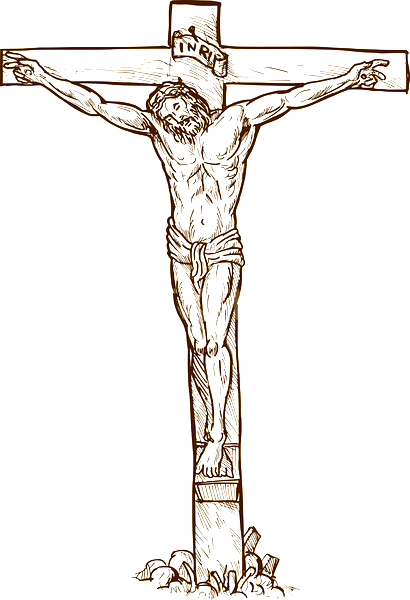
\includegraphics{cross.png}
	\end{figure}
	\clearpage
	\subsection{KANON MSZY ŚWIĘTEJ}
	\rub{Modlitwy Kanonu, którego pochodzenie sięga pierwszych wieków Kościoła, odzwierciedlają dokładnie myśl Apostołów i Zbawiciela. Dlatego powinniśmy z wielką czcią i radością odmawiać z kapłanem te modlitwy, które uświęciła tak starodawna tradycja.}
	
	\subsubsection{(Pierwsza) modlitwa wstawiennicza}
	\begin{parcolumns}[colwidths={2=3 in},nofirstindent]{2}
		\rub{Kapłan ogólnie poleciwszy ofiarę wstawia się (a) za cały Kościół wojujący (b) za biorących udział w Ofierze (c) w łączności z Kościołem tryumfującym. "Naprzód należy polecić ofiary i wtedy wygłosić imiona tych, których należy" (św. Innocenty I 417). Imiona odczytywano z tabliczek zwanych dyptychami. Wypisywano na nich imiona żywych i umarłych, których polecano modlitwom wiernych, oraz imiona świętych, których przy ofierze w dniu danym wspominano.}
		
		\negr{Te Igitur --- ogólne polecenie ofiar}
		
		\latin{Te igitur, clementissime Pater, per Iesum Christum Filium tuum Dominum nostrum, supplices rogamus ac petimus, uti accepta habeas, et benedicas haec (+) dona, haec (+) munera, haec (+) sancta sacrificia illibata.}
		\pol{Ciebie wiec, najmiłościwszy Ojcze, przez Jezusa Chrystusa Syna Twojego, Pana naszego, pokornie błagamy i prosimy: przyjmij te (+) dary, te (+) daniny, te (+) święte, nieskalane ofiary.}
		
		\negr{In Primis --- Za Kosciół wojujący}
		
		\latin{In primis, quae tibi offerimus pro Ecclesia tua sancta Catholica quam pacificare, custodire, adunare, et regere digneris toto orbe terrarum: una cum famulo tuo Papa nostro N. et Antistite nostro N. et omnibus orthodoxis, atque Catholicae et Apostolicae fidei cultoribus.}
		\pol{Składamy Ci je przede wszystkim za Kościół Twój Święty, powszechny: racz Go obdarzyć pokojem, strzec, jednoczyć i rządzić Nim na całym okręgu ziemskim, wraz ze sługą Twoim Papieżem naszym N., i Biskupem naszym N., i ze wszystkimi prawowiernymi powszechnej i apostolskiej wiary wyznawcami.}
		
		\negr{Memento --- za uczestników (wspomnienie żywych)}
		
		\latin{Memento, Domine famulorum, famularumque tuarum N. et N. et omnium circumstantium, quorum tibi fides cognita est, et nota devotio, pro quibus tibi offerimus: vel qui tibi offerunt hoc sacrificium laudis, pro se suisque omnibus: pro redemptione animarum suarum, pro spe salutis et incolumitatis suae: tibique reddunt vota sua aeterno Deo, vivo et vero.}
		\pol{Pomnij, Panie na sługi i służebnice Twoje N.N. i na wszystkich tu obecnych, których wierność jest Ci wiadoma, a gorliwość znana, za których Tobie ofiarujemy i którzy Ci składają tę ofiarę uwielbienia za siebie samych i za wszystkich swoich, za odkupienie dusz swoich, w nadziei zbawienia i ocalenia swego, oddając dary swoje, Tobie, Bogu wiecznemu, żywemu i prawdziwemu.}
		
		\negr{Communicantes --- w łączności z Kościołem tryumfującym}
		
		\latinS{Communicantes, et memoriam venerantes, in primis gloriosae semper virginis Mariae, Genitricis Dei et Domini nostri Iesu Christi: sed {et beati Ioseph, eiusdem virginis Sponsi} et beatorum Apostolorum ac Martyrum tuorum, Petri et Pauli, Andreae, Iacobi, Ioannis, Thomae, Iacobi, Philippi, Bartholomaei, Matthaei, Simonis et Thaddaei: Lini, Cleti, Clementis, Xysti, Cornelii, Cypriani, Laurentii, Chrysogoni, Ioannis et Pauli, Cosmae et Damiani, et omnium sanctorum tuorum: quorum meritis precibusque concedas, ut in omnibus protectionis tuae muniamur auxilio. Per eumdem Christum Dominum nostrum. Amen.}
		\polK{W świętym obcowaniu, ze czcią wspominamy przede wszystkim wsławioną zawsze Dziewicę Maryję, Rodzicę Boga, Pana naszego, Jezusa Chrystusa, a także Świętych Apostołów i Męczenników Twoich: (Apostołów) Piotra i Pawła, Andrzeja, Jakuba Jana, Tomasza, Jakuba, Filipa, Bartłomieja, Mateusza, Szymona, i Tadeusza, (Papieży) Linusa, Kleta, Klemensa, Ksystusa, Korneliusza, (Męczenników Cypriana, Wawrzyńca, Chryzogona, Jana i Pawła, Kosmę i Damiana, i wszystkich Świętych Twoich: racz dla ich zasług i modlitw wspierać nas w każdej potrzebie pomocą Swojej opieki. Przez tegoż Chrystusa, Pana naszego. Amen.}
	\end{parcolumns}
	
	\subsubsection{Hanc Igitur --- prośba o przyjęcie ofiary}
	\begin{parcolumns}[colwidths={2=3 in},nofirstindent]{2}
		\rub{Kapłan wyciąga dłonie nad Hostią i kielichem, a gdy zaczyna błogosławić, ministrant dzwoni, wierni klękają.}
		
		\latin{Hanc igitur oblationem servitutis nostrae, sed et cunctae familiae tuae, quaesumus, Domine, ut placatus accipias: diesque nostros in tua pace disponas, atque ab aeterna damnatione nos eripi, et in electorum tuorum iubeas grege numerari. Per Christum Dominum nostrum. Amen.}
		\pol{Prosimy Cię przeto, Panie, abyś tę ofiarę sług Twoich i całej rodziny Twojej miłościwie przyjął, dni życia naszego w pokoju swym ustalił i zechciał od wiecznego potępienia nas wybawić i zaliczyć w poczet wybranych Twoich. Przez Chrystusa, Pana naszego. Amen.}
	\end{parcolumns}
	
	\subsubsection{Quam Oblationem --- Prośba o przeistoczenie}
	\begin{parcolumns}[colwidths={2=3 in},nofirstindent]{2}
		\rub{Kulminacyjnym punktem w Ofierze Mszy Świętej jest przeistoczenie chleba i wina w Ciało i Krew Pańską. Ofiara, które się spełnia na ołtarzu, jest tą ofiarą, która się dokonała na Kalwarii. Ten sam Kapłan i Ofiara ta sama. Wzbudźmy w sobie wiarę w obecność Chrystusa pod postaciami chleba i wina mówiąc po cichu, podczas podniesienia słowa św. Tomasza: Pan Bóg i Bóg mój. (7 lat odp. dla tych, co mówią codzień odp. zup. raz na tydzień pod zwykłymi warunkami. S. Pen. 26, I, 1937)}
		
		\latin{Quam oblationem tu, Deus, in omnibus, quaesumus benedictam (+), adscriptam (+), ratam (+), rationabilem, acceptabilemque facere digneris: ut nobis Corpus (+), et Sanguis (+) fiat dilectissimi Filii tui, Domini nostri Iesu Christi.}
		\pol{Wsród wszystkich ofiar, prosimy Cię, Ty Boże, racz te pobło+gosławić, u+znać, za+twierdzić, prawdziwą i miłą sobie uczynić, tak, żeby stała się dla nas Cia+łem i Krwią (+) najmilszego Syna Twojego, Pana naszego, Jezusa Chrystusa.}
	\end{parcolumns}
	
	\subsubsection{Konsekracja chleba}
	\begin{parcolumns}[colwidths={2=3 in},nofirstindent]{2}
		\rub{Kapłan bierze do rak Hostię}
		
		\latin{Qui pridie quam pateretur, accepit panem in sanctas ac venerabiles manus suas: et elevatis oculis in coelum ad te Deum Patrem suum omnipotentem, tibi gratias agens, benedixit (+), fregit, deditque discipulis suis, dicens: Accipite, et manducate ex hoc omnes:}
		\pol{Który w przedzień Swej Męki wziął chleb w święte i czczigodne ręce Swoje, a wzniósłszy oczy ku niebu do Ciebie, Boga, Ojca Swego wszechmogącego, Tobie czyniąc dzięki, poblogo+sławił, połamał i rozdał uczniom Swoim, mówiąc: Bierzcie i jedzcie z tego wszyscy:}
		
		\rub{Kapłan pochyla się nad Hostią}
		
		\latin{\textbf{HOC EST ENIM CORPUS MEUM}}
		\pol{\textbf{TO JEST BOWIEM CIAŁO MOJE}}
		
		\rub{Gdy kapłan podnosi Hostię Najświętszą, ministrant dzwoni, a wierni adorują w ciszy.}
	\end{parcolumns}
	
	\subsubsection{Konsekracja wina}
	\begin{parcolumns}[colwidths={2=3 in},nofirstindent]{2}
		\rub{Kapłan bierze do rąk Kielich.}
		
		\latin{Simili modo postquam coenatum est, accipiens et hunc praeclarum Calicem in sanctas ac venerabiles manus suas: item tibi gratias agens, bene + dixit, deditque discipulis suis, dicens: Accipite, et bibite ex eo omnes.}
		\pol{Podobnież, gdy było po wieczerzy, ujmując i ten przesławny Kielich w święte i czcigodne ręce Swoje, również dzięki Tobie czyniąc, poblogo+sławił i podał uczniom Swoim, mówiąc: Bierzcie i pijcie z niego wszyscy:}
		
		\rub{Kapłan pochyla się nad Kielichem.}
		
		\latin{\textbf{HIC EST ENIM CALIX SANGUINIS MEI, NOVI ET AETERNI TESTAMENTI: QUI PRO VOBIS ET PRO MULTIS EFFUNDETUR IN REMISSIONEM PECCATORUM.}}
		\pol{\textbf{TO JEST BOWIEM KIELICH KRWI MOJEJ, NOWEGO I WIECZNEGO PRZYMIERZA: KTÓRY ZA WAS I ZA WIELU WYLANY BĘDZIE NA ODPUSZCZENIE GRZECHÓW.}}
		
		\latin{Haec quotiescumque feceritis, in mei memoriam facietis.}
		\pol{To ile razy czynić będziecie, na moją czyńcie pamiątkę.}
		
		\rub{Gdy kapłan podnosi kielich, ministrant dzwoni. Wierni adorują w ciszy Krew Przenajświętszą}
	\end{parcolumns}
	
	\subsubsection{Unde Et Memores --- Wspomnienie Tajemnicy Odkupienia (Anamneza)}
	\begin{parcolumns}[colwidths={2=3 in},nofirstindent]{2}
		\rub{Pamiątka Chrystusa, to nie tylko czcze wspomnienie, ale rzeczywiste uobecnienie całej Tajemnicy Odkupienia --- co też podkreśla natychmiast kapłan w następnej modlitwie zwanej "anamneza" czyli "wspomnienie".}
		
		\latinS{Unde et memores Domine, nos servi tui, sed et plebs tua sancta, eiusdem Christi Filii tui Domini nostri, tam beatae passionis, nec non et ab inferis resurrectionis, sed et in caelos gloriosae ascensionis: offerimus praeclarae majestati tuae de tuis donis ac datis, hostiam (+) puram, hostiam (+) sanctam, hostiam (+) immaculatam, Panem (+) sanctum vitae aeternae, et Calicem (+) salutis perpetuae.}
		\polK{Przeto i my słudzy Twoi, Panie, oraz lud Twój święty, wspominając tak błogosławioną Mękę, jak też i Zmartwychwstanie z otchłani i chwalebne Wniebowstąpienie tegoż Chrystusa, Syna Twojego, Pana naszego, ofiarujemy przedostojnemu Majestatowi Twojemu, z darów i dobrodziejstw Twoich, Hostię (+) czystą, Hostię (+) świetą, Hostię (+) Niepokalaną, Chleb (+) święty wiekuistego życia i Kielich (+) zbawienia wiecznego.}
	\end{parcolumns}
	
	\subsubsection{Supra Quae --- Modlitwa o przyjęcie Ofiary bezkrwawej}
	\begin{parcolumns}[colwidths={2=3 in},nofirstindent]{2}
		\rub{Bóg łaskawie przyjął ofiary Starego Zakonu, które były tylko figurą Ofiary Chrystusa; o ile bardziej przychylnie raczy wejrzeć na ofiarę Nowego Przymierza.}
		
		\latinS{Supra quae propitio ac sereno vultu respicere digneris: et accepta habere, sicuti accepta habere dignatus es munera pueri tui iusti Abel, et sacrificium patriarchae nostri Abrahae: et quod tibi obtulit summus sacerdos tuus Melchisedech, sanctum sacrificium, immaculatam hostiam.}
		\polK{Racz na nie wejrzeć przejednanym i łaskawym obliczem i przyjąć je tak mile, jak mile przyjąć raczyłeś dary sprawiedliwego sługi Twego Abla i ofiarę Patryjarchy naszego Abrahama i tę, którą Ci złożył najwyższy Twój Kapłan Melchizedek, ofiarę świętą, hostię niepokalaną.}
	\end{parcolumns}
	
	\subsubsection{Druga modlitwa wstawiennicza}
	\begin{parcolumns}[colwidths={2=3 in},nofirstindent]{2}
		\rub{Kapłan pochylony nad ołtarzem, modli się o łaski dla uczestników Ofiary. Owym aniołem, który ma ofiarę przedstawić jest sam Chrystus. Według innych jest nim Duch Święty lub jakiś anioł ofiarnik. }
		
		\negr{Supplices --- za uczestników Ofiary}
		
		\latin{Supplices te rogamus, omnipotens Deus; iube haec perferri per manus sancti Angeli tui in sublime altare tuum, in conspectu divinae majestatis tuae: ut quotquot ex hac altaris participatione, sacrosanctum Filii tui Corpus (+) et Sanquinem (+) sumpserimus omni benedictione caelesti et gratia repleamur. Per eumdem Christum, Dominum nostrum. Amen.}
		\pol{Pokornie Cię błagamy, wszechmogący Boże, rozkaz, by ręce świętego Anioła Twego zaniosły tę Ofiarę na niebiański Twój ołtarz, przed oblicze Boskiego Majestatu Twego, abyśmy wszyscy, tego ołtarza uczestnicy, pożywając przenajświętsze + Ciało i Krew + Syna Twego, otrzymali z niebios pełnię błogosławieństwa i łaski. Przez tegoż Chrystusa, Pana naszego. Amen.}
		
		\negr{Memento --- za zmarłych}
		
		\latin{Memento etiam, Domine, famulorum famularumque tuarum N. et N. qui nos praecesserunt cum signo fidei, et dormiunt in somno pacis.\\Ipsis, Domine, et omnibus in Christo quiescentibus, locum refrigerii, lucis et pacis, ut indulgeas, deprecamur. Per eumdem Christum Dominum nostrum. Amen.}
		\pol{Pomnij też, Panie, na sługi i służebnice Twoje NN., którzy nas wyprzedzili ze znamieniem wiary i śpią snem pokoju.\\Błagamy Cię, Panie, użycz im i wszystkim tym, którzy w Chrystusie spoczywają, miejsca ochłody, światła i pokoju. Przez tegoż Chrystusa, Pana naszego. Amen.}
		
		\negr{Nobis Quoque Peccatoribus --- w łącznosci z Kościołem tryumfującym }
		
		\rub{Kapłan bije się w piersi, ministrant raz dzwoni.}
		
		\latin{Nobis quoque peccatoribus famulis tuis, de multitudine miserationum tuarum sperantibus, partem aliquam et societatem donare digneris, cum tuis sanctis Apostolis et Martyribus: cum Ioanne, Stephano, Matthia, Barnaba, Ignatio, Alexandro, Marcellino, Petro, Felicitate, Perpetua, Agatha, Lucia, Agnete, Caecilia, Anastasia, et omnibus sanctis tuis: intra quorum nos consortium, non aestimator meriti, sed veniae, quaesumus, largitor admitte. Per Christum Dominum nostrum.}
		\pol{Nam także, grzesznym sługom Twoim, którzy pokładamy nadzieję w mnóstwie litości Twojej, racz dać jakiś udział i obcowanie ze świętymi Twoimi Apostołami i Męczennikami: Janem (Chrzcicielem), Szczepanem (Diakonem), Maciejem (Apostołem), Barnabą, Ignacym (Biskupem) Aleksandrem, Marcelinem, Piotrem, (Męczennice) Felicytą, Perpetuą, Agatą, Łucją, Agnieszką, Cecylią, Anastazją, i całym gronem Twych Świętych; dopuść nas, prosimy, do ich współdziedzictwa, nie z naszych zasług biorąc miarę, lecz przebaczeniem obdarzając Przez Chrystusa, Pana naszego.}
	\end{parcolumns}
	
	\subsubsection{Zakończenie}
	\begin{parcolumns}[colwidths={2=3 in},nofirstindent]{2}
		\latin{Per quem haec omnia, Domine, semper bona creas, sanctificas (+), vivificas (+), benedicis (+) et praestas nobis.}
		\pol{Przez Niego, Panie, te wszystkie dary zawsze dobrymi stwarzasz, uswię+casz, oży+wiasz, błogo+sławisz i nam ich udzielasz.}
		
		\rub{Kapłan odkrywa kielich i czyni Hostią Św. pięć razy znak krzyża, po czym podnosi kielich wraz z Hostią (małe podniesienie). Jednocześnie wielbi Boga, mówiąc:}
		
		\latin{Per ipsum (+), et cum ipso (+), et in ipso (+), est tibi Deo Patri (+) omnipotenti, in unitate Spritus (+) Sancti, omnis honor et gloria.}
		\pol{Przez + Niego i z + Nim, i w + Nim masz, Boże Ojcze + wszechmogący, w jedności Ducha + Świętego, wszelką cześć i chwałę.}
		\latinS{Per omnia saecula saeculorum.}
		\polK{Przez wszystkie wieki wieków. }
		\latinM{Amen.}
		\polW{Amen.}
	\end{parcolumns}
	
	
	\subsection{CZĘŚĆ TRZECIA}
	
	\subsubsection{Pater Noster --- Modlitwa Pańska}
	\begin{parcolumns}[colwidths={2=3 in},nofirstindent]{2}
		\rub{Teraz po złożeniu Ofiary, następuje uczta. W odpowiedzi na nasze dary, prośby i błagania Bóg udzieli nam pokarmu świętego, w którym są zawarte wszystkie łaski i dobrodziejstwa, bo pokarm ten, to sam Pan Jezus pod postaciami chleba i wina. Jest to stwierdzenie, ze Bóg nas wysłuchał i chce nam dopomóc, jako swym dzieciom. Jako przygotowanie do Komunii św. odmówmy z głębi serca "Ojcze nasz" i prośmy Pana Jezusa, aby to Jego Ciało, które spożywać będziemy, stało się nam lekarstwem dla duszy i ciała.}
		
		\latinS{Oremus. Praeceptis salutaribus moniti, et divina institutione formati, audemus dicere:\\Pater noster, qui es in caelis, sanctificetur nomen tuum. Adveniat regnum tuum. Fiat voluntas tua, sicut in caelo et in terra. Panem nostrum quotidianum da nobis hodie. Et dimitte nobis debita nostra, sicut et nos dimittimus debitoribus nostris. Et ne nos inducas in tentationem.}
		\polK{Módlmy się. Nauką zbawienną zachęceni i Boskim ustanowieniem przygotowani, ośmielamy się mówić:\\Ojcze nasz, Któryś jest w niebie, święć się Imię Twoje. Przyjdź królestwo Twoje, Bądź wola Twoja, jako w niebie tak i na ziemi: Chleba naszego powszedniego daj nam dzisiaj. I odpuść nam nasze winy, jako i my odpuszczamy naszym winowajcom. I nie wódź nas na pokuszenie.}
		\latinM{Sed libera nos a malo.}
		\polW{Ale nas zbaw ode złego.}
		\latinS{Amen.}
		\polK{Amen.}
		
		\rub{Kapłan rozwija ostatnią prośbę:}
		
		\negr{Libera Nos}
		
		\latin{Libera nos, quaesumus, Domine, ab omnibus malis, praeteritis, praesentibus et futuris: et intercedente beata et gloriosa semper Virgine Dei Genitrice Maria, cum beatis Apostolis tui Petro et Paulo, atque Andrea, et omnibus Sanctis, da propitius pacem in diebus nostris: ut, ope misericordiae tuae adiuti, et a peccato simus semper liberi et ab omni perturbatione securi. Per eumden Dominum nostrum Iesum Christum, Filium tuum. Qui tecum vivit et regnat in unitate Spiritus Sancti Deus. Per omnia saecula saeculorum. Amen.}
		\pol{Wybaw nas, prosimy Cię, Panie od wszelkich nieszczęść przeszłych, obecnych i przyszłych, a za przyczyną Najświętszej i chwalebnej zawsze Dziewicy, Bogarodzicy Maryi, świętych Apostołów Twoich Piotra i Pawła, oraz Andrzeja i wszystkich Świętych, udziel nam miłościwie pokoju za dni naszych, abyśmy wsparci pomocą miłosierdzia Twego i od grzechu byli zawsze wolni i od wszelkiej trwogi bezpieczni. Przez tegoż Pana naszego Jezusa Chrystusa, Syna Twojego, który z Tobą żyje i króluje w jedności Ducha Świętego Bóg, przez wszystkie wieki wieków. Amen. }
	\end{parcolumns}
	
	\subsubsection{Łamanie Chleba i modły o pokój}
	\begin{parcolumns}[colwidths={2=3 in},nofirstindent]{2}
		\rub{Obrzęd Łamania Chleba jest również symbolem gwałtownej śmierci Chrystusa, połączenie zaś Hostii z Krwią wskazuje na Jego zmartwychwstanie. Pierwszym owocem Eucharystii jest pokój, czyli jedność z Bogiem i jedność między nami.}
		
		\latinS{Per omnia saecula saeculorum.}
		\polK{Przez wszystkie wieki wieków. }
		\latinM{Amen.}
		\polW{Amen.}
		\latinS{Pax (+) Domini sit (+) semper vobiscum (+).}
		\polK{Pokój (+) Pana niech (+) będzie zawsze z wami (+).}
		\latinM{Et cum spiritu tuo.}
		\polW{I z duchem twoim.}
		
		\rub{Kapłan wpuszcza cząstkę Hostii Św. do Kielicha, mówiąc}
		
		\latinS{Haec commixtio et consecratio Corporis at Sanguinis Domini nostri Iesu Christi fiat accipientibus nobis in vitam aeternam. Amen.}
		\polK{To połączenie i poświecenie Ciała i Krwi Pana naszego, Jezusa Chrystusa, niech się nam, którzy je przyjmujemy, przyczyni do żywota wiecznego. Amen.}
		
		\negr{Agnus Dei --- Baranku Boży}
		
		\rub{Pochylając się i uderzając się trzykroć w piersi, kapłan mówi:}
		
		\latinS{Agnus Dei, qui tollis peccata mundi, miserere nobis.\\Agnus Dei, qui tollis peccata mundi, miserere nobis.\\Agnus Dei, qui tollis peccata mundi, dona nobis pacem.}
		\polK{Baranku Boży, który gładzisz grzechy świata, zmiłuj się nad nami.\\Baranku Boży, który gładzisz grzechy świata, zmiłuj się nad nami.\\Baranku Boży, który gładzisz grzechy świata, obdarz nas pokojem.}
	\end{parcolumns}
	
	\subsubsection{Modlitwy przed Komunią}
	\begin{parcolumns}[colwidths={2=3 in},nofirstindent]{2}
		\rub{Następują trzy ciche prywatne modlitwy kapłana, pięknie przypominające skutki, jakie Komunia ma spowodować w duszach naszych: pokój, uzdrowienie, łaskę Bożą. Opieramy się w tej chwili na zasługach Chrystusa i wierze Kościoła.}
		
		\negr{Domine Iesus Christe I}
		
		\latin{Domine Iesu Christe, qui dixisti Apostolis tuis: pacem relinquo vobis, pacem meam do vobis: ne respicias peccata mea, sed fidem Ecclesiae tuae; eamque secundum voluntatem tuam pacificare et coadunare digneris. Qui vivis et regnas Deus, per omnia saecula saeculorum. Amen.}
		\pol{Panie Jezu Chryste, któryś rzekł Apostołom Twoim: pokój wam zostawiam, pokój Mój wam daję, patrz nie na grzechy moje, lecz na wiarę Twojego Kościoła, i racz go według Twej woli obdarzać pokojem i w jedności umacniać, który żyjesz i królujesz, Bóg przez wszystkie wieki wieków. Amen.}
		
		\negr{Domine Iesu Christe II}
		
		\latin{Domine Iesu Christe, Fili Dei vivi, qui ex voluntate Patris cooperante Spritu Sancto, per mortem tuam mundum vivificasti: libera me per hoc sacrosanctum Corpus et Sanguinem tuum ab omnibus iniquitatibus meis et universis malis: et fac me tuis semper inhaerere mandatis: et a te nunquam separari permittas: qui cum eodem Deo Patre et Spiritu Sancto vivis et regnas Deus in saecula saeculorum. Amen.}
		\pol{Panie Jezu Chryste, Synu Boga żywego, który z woli Ojca za sprawa Ducha Świętego, przez śmierć Swoją świat ożywiłeś, wybaw mnie przez to Przenajświętsze Ciało i Krew Twoją od wszelkich nieprawości moich i od wszelkiego zła i spraw, bym zawsze strzegł przykazań Twoich i nie dozwól, bym się kiedykolwiek odłączył od Ciebie, który z tymże Ojcem i Duchem Świętym żyjesz i królujesz, Bóg na wieki wieków. Amen.}
		
		\negr{Perceptio Corporis}
		
		\latin{Perceptio Corporis tui, Domine Iesu Christe, quod ego indignus sumere praesumo, non mihi proveniat in iudicium et condemnationem: sed pro tua pietate prosit mihi ad tutamentum mentis et corporis, et ad medelam percipiendam. Qui vivis et regnas cum Deo Patre in unitate Spiritus Sancti Deus, per omnia saecula saeculorum. Amen.}
		\pol{Przyjęcie Ciała Twego, Panie Jezu Chryste, które ja, niegodny sługa, spożywać się ważę, niechaj mi się nie obróci na sąd i potępienie, lecz niechaj raczej posłuży mi ku obronie i uzdrowieniu duszy i ciała: który żyjesz i królujesz z Bogiem Ojcem w jedności Ducha Świętego Bóg, przez wszystkie wieki wieków. Amen.}
	\end{parcolumns}
	
	\subsubsection{Komunia kapłana}
	\begin{parcolumns}[colwidths={2=3 in},nofirstindent]{2}
		\rub{Kapłan przyklęka, bierze do rąk Hostię św., aby ją przyjąć i mówi:}
		
		\latin{Panem caelestem accipiam et nomen Domini invocabo.}
		\pol{Chleb niebiański przyjmę i wezwę Imienia Pana.}
		
		\rub{Trzymając Hostię Świętą w lewej dłoni, kapłan uderza się w piersi trzy razy, a ministrant dzwoni:}
		
		\latin{Domine, non sum dignus ut intres sub tectum meum: sed tantum dic verbo, et sanabitur anima mea (ter.)}
		\pol{Panie, nie jestem godzien, abyś wszedł do wnętrza mego, ale rzeknij tylko słowem, a będzie uzdrowiona dusza moja. (trzykrotnie)}
		
		\rub{Trzymając Hostię Świętą w prawej ręce, kapłan czyni Nią znak krzyża i mówi:}
		
		\latin{Corpus Domini nostri Iesu Christi custodiat animam meam in vitam aeternam. Amen.}
		\pol{Ciało Pana naszego Jezusa Chrystusa niechaj strzeże duszy mojej na żywot wieczny. Amen.}
		
		\rub{Po chwili kapłan bierze do rąk Kielich i modli się słowami psalmu, który Chrystus odmawiał w czasie Ostatniej Wieczerzy:}
		
		\latin{Quid retribuam Domino pro omnibus, quae retribuit mihi? Calicem salutaris accipiam, et nomen Domini invocabo. Laudans invocabo Dominum, et ab inicimcis meis salvus ero.\\Sanguis Domini nostri Jesu Christi custodiat animam meam in vitam aeternam. Amen.}
		\pol{Cóż zwrócę Panu za wszystko, co dla mnie uczynił; Kielich zbawienia wezmę i wezwę Imienia Pana. Wielbiąc zawołam do Pana i od nieprzyjaciół moich będę ocalony.\\Krew Pana naszego Jezusa Chrystusa niechaj strzeże duszy mojej na żywot wieczny. Amen.}
	\end{parcolumns}
	
	\subsubsection{Komunia wiernych}
	\begin{parcolumns}[colwidths={2=3 in},nofirstindent]{2}
		\rub{Kapłan zwraca się do wiernych z Cyborium i trzymając Hostię Świętą, mówi:}
		
		\latin{Ecce Agnus Dei, ecce Qui tollit peccata mundi.}
		\pol{Oto Baranek Boży: oto, który gładzi grzechy świata}
		
		\rub{Bij się w piersi za każdym razem i mów wraz z ministrantem (kapłanem):}
		
		\latin{Domine, non sum dignus ut intres sub tectum meum: sed tantum dic verbo, et sanabitur anima mea (ter.)}
		\pol{Panie, nie jestem godzien, abyś wszedł do wnętrza mego, ale rzeknij tylko słowem, a będzie uzdrowiona dusza moja. (trzykrotnie)}
		
		\rub{Podając Komunię Świętą, kapłan mówi:}
		
		\latin{Corpus Domini nostri Iesu Christi custodiat animam tuam in vitam aeternam. Amen.}
		\pol{Ciało Pana naszego Jezusa Chrystusa niechaj strzeże duszy Twojej na żywot wieczny. Amen.}
		
		\rub{Gdy wszyscy otrzymali Komunie Świętą, kapłan powraca na ołtarz i umieszcza Cyborium w Tabernakulum. }
	\end{parcolumns}
	
	\subsubsection{Dziękczynienie}
	\begin{parcolumns}[colwidths={2=3 in},nofirstindent]{2}
		\rub{Po czym ministrant bierze ampułki i nalewa wina do kielicha. Kapłan modli się:}
		
		\latin{Quod ore sumpsimus Domine, pura mente capiamus: et de munere temporali fiat nobis remedium sempiternum.}
		\pol{Cośmy usty spożyli, Panie, daj czystym przyjąć umysłem, a dar ten doczesny niech się nam stanie lekarstwem na wieczność}
		
		\rub{Ministrant polewa palce kapłana winem i wodą --- Kapłan modli się.}
		
		\latin{Corpus tuum, Domine, quod sumpsi, et Sanguis, quem potavi, adhaereat visceribus meis: et praesta, ut in me non remaneat scelerum macula, quem pura et sancta refecerunt sacramenta. Qui vivis et regnas in saecula saeculorum. Amen.}
		\pol{Ciało Twe, Panie, które spożyłem, i Krew, którą wypiłem, niech przywrze do mego wnętrza, i spraw, aby zmaza grzechów nie została we mnie, którego czyste i święte posiliły Sakramenta. Który żyjesz i królujesz na wieki wieków. Amen.}
		
		\rub{Kapłan wyciera kielich i przykrywa go welonem. --- Ministrant przenosi Mszał. }
	\end{parcolumns}
	
	\subsubsection{Communio --- Śpiew przy Komunii}
	\rub{Po czym kapłan przechodzi na stronę Lekcji i odczytuje Komunię.}
	
	\subsubsection{Postcommunio --- Modlitwy po Komunii}
	\begin{parcolumns}[colwidths={2=3 in},nofirstindent]{2}
		\latinS{Dominus vobiscum.}
		\polK{Pan z wami.}
		\latinM{Et cum spiritu tuo.}
		\polW{I z duchem Twoim.}
		\latinS{Oremus.}
		\polK{Módlmy sie.}
		
		\rub{Kapłan odczytuje modlitwę Postcommunio. Dziękujmy razem z kapłanem Panu Bogu, że nas raczył posilić Ciąłem Syna Swego Jezusa Chrystusa i prośmy, aby ta Komunia Św. dała nam siłę do spełnienia naszych obowiązków i doprowadziła do życia wiecznego przez tegoż Chrystusa, Pana naszego, który z Bogiem Ojcem żyje i króluje w jedności Ducha Świętego.}
		
		\latinS{Per omnia saecula saeculorum.}
		\polK{Przez wszystkie wieki wieków. }
		\latinM{Amen.}
		\polW{Amen.}
		
		\rub{Po skończonych modlitwach kapłan wraca na środek ołtarza, całuje go i zwracając się do wiernych, mówi:}
		
		\latinS{Dominus vobiscum.}
		\polK{Pan z wami.}
		\latinM{Et cum spiritu tuo.}
		\polW{I z duchem Twoim.}
		\latinS{Ite, missa est.}
		\polK{Idźcie, Msza się skończyła.}
		\latinM{Deo gratias.}
		\polW{Bogu niech będą dzięki.}
	\end{parcolumns}
	
	\subsubsection{Placeat Tibi --- Ostatnia modlitwa}
	\begin{parcolumns}[colwidths={2=3 in},nofirstindent]{2}
		\rub{Pochylając się nad ołtarzem, kapłan mówi:}
		
		\latin{Placeat tibi, sancta Trinitas, obsequium servitutis meae: et praesta, ut sacrificium quod oculis tuae maiestatis indignus obtuli, tibi sit acceptabile, mihique, et omnibus pro quibus illud obtuli, sit te miserante propitiabile. Per Christum Dominum nostrum. Amen.}
		\pol{O Trójco Przenajświętsza, niechaj Ci miłym będzie hołd służby mojej i spraw aby ta ofiara, którą ja niegodny zaniosłem przed oczy majestatu Twego, była Tobie przyjemna, mnie zaś i wszystkim, za których ją złożyłem, stała się przejednaniem dzięki Twemu miłosierdziu. Przez Chrystusa Pana naszego. Amen.}
		
		\negr{Błogosławieństwo}
		
		\rub{Kapłan całuje ołtarz, a na słowo "Pater" odwraca się do wiernych.}
		
		\latinS{Benedicat vos omnipotens Deus, Pater, et Filius (+), et Spiritus Sanctus.}
		\polK{Niech was błogosławi wszechmogący Bóg, Ojciec i Syn (+), i Duch Święty.}
		\latinM{Amen.}
		\polW{Amen.}
	\end{parcolumns}
	
	\subsubsection{Ostatnia Ewangelia}
	\begin{parcolumns}[colwidths={2=3 in},nofirstindent]{2}
		\rub{Kapłan przechodzi na stronę Ewangelii. Czyni znak krzyża najpierw na ołtarzu, potem na swym czole, ustach i sercu.}
		
		\latinS{Dominus vobiscum.}
		\polK{Pan z wami.}
		\latinM{Et cum spiritu tuo.}
		\polW{I z duchem Twoim.}
		\latinS{(+) Initium sancti Evangelii secundum Ioannem.}
		\polK{(+) Początek świętej Ewangelii według Świętego Jana.}
		\latinM{Gloria tibi Domine.}
		\polW{Chwała Tobie Panie.}
		\latin{In prinicipio erat Verbum, et Verbum erat apud Deum, et Deus erat Verbum. Hoc erat in principio apud Deum. Omnia per ipsum facta sunt, et sine ipso factum est nihil, quod factum est. In ipso vita erat, et vita erat lux hominum: et lux in tenebris lucet, et tenebrae eam non comprehenderunt.\\Fuit homo missus a Deo, cui nomen erat Ioannes. Hic venit in testimonium, ut testimonium perhiberet de lumine, ut omnes crederent per illum. Non erat ille lux, sed ut testimonium perhiberet de lumine.\\Erat lux vera, quae illuminat omnem hominem venientem in hunc mundum. In mundo erat, et mundus per ipsum factus est, et mundus eum non cognovit. In propria venit, et sui eum non receperunt. Quotquot autem receperunt eum, dedit eis potestatem filios Dei fieri, his qui credunt in nomine eius. Qui non ex sanguinibus, neque ex voluntate carnis, neque ex voluntate viri, sed ex Deo nati sunt.\\\rub{(hic genuflectitur)} ET VERBUM CARO FACTUM EST, et habitavit in nobis et vidimus gloriam eius, gloriam quasi Unigeniti a Patre, plenum gratiae et veritatis.}
		\pol{Na początku było Słowo, a Słowo było u Boga, a Bogiem było Słowo. Ono to było na początku u Boga. Wszystko przez nie się stało, a bez Niego nic się nie stało, co się stało. W Nim było życie, a Życie było Światłością ludzi, a Światłość w ciemnościach świeci, a ciemności Jej nie ogarnęły.\\Był człowiek posłany od Boga, a na imię mu było Jan. Ten przyszedł na świadectwo, aby świadectwo dąć o Światłości, aby przezeń wszyscy uwierzyli. Nie był on Światłością, ale miął świadczyć o Światłości.\\Było Światło prawdziwe, które oświeca każdego człowieka, gdy na ten świat przychodzi. Ono było na świecie, a świat przez nie został uczynion, a świat Go nie poznał. Do swego przyszło, a swoi Go nie przyjęli. Tym zaś wszystkim, którzy Go przyjęli, dało moc, by się stali synami Bożymi, tym co wierzą w Imię Jego, którzy nie ze krwi, ani z pożądliwości ciała, ani z woli męża, ale z Boga się narodzili.\\\rub{(tu wszyscy klękają)} A SŁOWO CIAŁEM SIĘ STAŁO i mieszkało między nami. I oglądaliśmy chwałę Jego, chwale jako Jednorodzonego od Ojca, pełnego łaski i prawdy.}
		\latinM{Deo gratias.}
		\polW{Bogu niech będą dzięki.}
	\end{parcolumns}
	
	\section{MODLITWY PO KAŻDEJ CICHEJ MSZY ŚWIĘTEJ}
	\begin{parcolumns}[colwidths={2=3 in},nofirstindent]{2}
		\textit{Przez Ojca Św. Leona XIII przepisane}
		
		\textit{\rub{Po cichej Mszy Św., kapłan klęcząc u stopni ołtarza, mówi z wiernymi poniższe modlitwy. Zaleca się wiernym samodzielne odmawianie tych modlitw także po Mszach Św. uroczystych.}}
		
		\negr{Salutatio Angelica --- Pozdrowienie Anielskie}
		
		\latin{Ave Maria (ter)}
		\pol{Zdrowaś Maryjo (trzy razy)}
		
		\negr{Antyfona}
		
		\latin{Salve Regina, Mater misericordiae. Vita, dulcedo, et spes nostra, salve. Ad te clamamus exsules filii Hevae. Ad te Suspiramus, gementes et flentes in hac lacrimarum valle. Eia ergo, Advocata nostra, illos tuos misericordes oculos ad nos converte. Et Iesum, benedictum fructum ventris tui, nobis post hoc exsilium ostende. O clemens, o pia, o dulcis Virgo Maria.}
		\pol{Witaj Królowo, Matko miłosierdzia, życie słodyczy i nadziejo nasza, witaj! Do Ciebie wołamy, wygnańcy, synowie Ewy. Do Ciebie wzdychamy, jęcząc i płacząc na tym łez padole. Racz przeto, Orędowniczko nasza, miłosierne oczy twoje zwrócić na nas i na Jezusa, błogosławiony owoc żywota twego okaz nam po tym wygnaniu. O łaskawa, o litościwa, o słodka Panno Maryjo!}
		
		\latinV{Ora pro nobis, sancta Dei Genitrix. }
		\polV{Módl się za nami świętą Boża Rodzicielko. }
		\latinR{Ut digni efficiamur promissionibus Christi.}
		\polR{Abyśmy się stali godnymi obietnic Pana Chrystusowych.}
		
		\latin{Oremus. Deus refugium nostrum et virtus, populum ad te clamantem propitius respice; et intercedente gloriosa et immaculata Virgine Dei Genitrice Maria, cum beato Iosepho eius Sponso, ac beatis Apostolis tuis Petro et Paulo, et omnibus Sanctis, quas pro conversione peccatorum, pro libertate et exaltatione sanctae Matris Ecclesiae, preces effundimus, misericors et benignus exaudi. Per eumden Christum, Dominum nostrum.}
		\pol{Módlmy się. Boże, ucieczko nasza i mocy, wejrzyj łaskawie na lud Twój do Ciebie wołający i za przyczyną chwalebnej i niepokalanej Dziewicy i Matki Bożej Maryi, z świętym jej Oblubieńcem Józefem, z świętymi Apostołami Twoimi Piotrem i Pawłem, oraz wszystkimi Świętymi, wysłuchaj miłościwie i łaskawie prośby nasze, które za nawrócenie grzeszników, za wolność i wywyższenie świętej Matki Kościoła naszego do Ciebie zanosimy. Przez tegoż Chrystusa, Pana naszego.}
		\latinR{ Amen.}
		\polR{ Amen.}
		
		\negr{Modlitwa do Św. Michała Archanioła (Egzorcyzm prywatny)}
		
		\latin{Sancte Michael Archangele, defende nos in proelio, contra nequitiam et insidias diaboli esto praesidium. Imperat illi Deus, supplices deprecamur: tuque, Princeps militiae caelestis, Satanam aliosque spiritus malignos, qui ad perditionem animarum pervagantur in mundo, divina virtute, in infernum detrude.}
		\pol{Święty Michale Archaniele! Wspomagaj nas w walce, a przeciw niegodziwości i zasadzkom złego ducha bądź naszą obroną. Oby go Bóg pogromić raczył, pokornie o to prosimy, a Ty, Wodzu niebieskich zastępów, Szatana i inne duchy złe, które na zgubę dusz ludzkich po tym świecie krążą, mocą Bożą strąć do piekła.}
		
		\latinR{Amen.}
		\polR{Amen.}
		
		\negr{Wezwanie do Najśw. Serca Pana Jezusa (dodane przez Św. Piusa X)}
		
		\latinV{Cor Iesu sacratissimum}
		\polV{Najswiętsze Serce Jezusa.}
		
		\latinR{Miserere nobis. (ter)}
		\polR{Zmiłuj sią nad nami! (trzy razy)}
	\end{parcolumns}

\end{document}
